%%%%%%%%%%%%%%%%%%%%%%%%%%%%%%%%%%%%%%%%%%%%%%%%%%%%%%%%%%%%%%%%%%%%%%%%%%%%%%%%%%%%
%%----------------------------------------------------------------------------------
% DO NOT Change this is the required setting A4 page, 11pt, onside print, book style
%%----------------------------------------------------------------------------------
\documentclass[a4paper,11pt,oneside]{book} 
\usepackage{CS_report} % DO NOT REMOVE THIS LINE. 
%%%%%%%%%%%%%%%%%%%%%%%%%%%%%%%%%%%%%%%%%%%%%%%%%%%%%%%%%%%%%%%%%%%%%%%%%%%%%%%%%%%%

%%%%%%%%%%%%%%%%%%%%%%%%%%%%%%%%%%%%%%%%%%%%%%%%%%%%%%%%%%%%%%%%%%%%%%%%%%%%%%%%%%%%
\begin{document}

    \captionsetup[figure]{margin=1.5cm,font=small,name={Figure},labelsep=colon}
    \captionsetup[table]{margin=1.5cm,font=small,name={Table},labelsep=colon}
    
    \frontmatter
    %%%%%%%%%%%%%%%%%%%%%%%%%%%%%%%%%%%%%%%%%%%%%%%%%%%%%%%%%%%%%%%%%%%%%%%%%%%%%%%%
    \begin{titlepage}      
        \begin{center}
            
\includegraphics[width=3cm]{figures/Universitaet_Logo_RGB.pdf}\\[0.5cm]
            {\LARGE Technical University Munich\\[0.5cm]
            School of Engineering and Design}\\[2cm]
			%{\color{blue} \rule{\textwidth}{1pt}}
			
			% -------------------------------
			% You need to edit some details here
			% -------------------------------  
            \linespread{1.2}\huge {
                %%%%%%%%%%%%%%%%%%%%%%%%%%%%
                %TODO: 1 TITLE of Your PROJECT 
                %%%%%%%%%%%%%%%%%%%%%%%%%%%%
                % change the following line                
                Report for Deep Learning for PDEs  in Engineering Physics
            
            }
            \linespread{1}~\\[2cm]
			%{\color{blue} \rule{\textwidth}{1pt}}
            {\Large 
                %%%%%%%%%%%%%%%%%%%%%%%%%%%%
                %TODO: 2 YOUR NAME
                %%%%%%%%%%%%%%%%%%%%%%%%%%%%             
                % change the following line
                Om Anant Kulkarni \\
                Student ID: 03812156
                % change end             
            }\\[1cm] 
            

            {\large 
                %%%%%%%%%%%%%%%%%%%%%%%%%%%%
                %TODO: 3 YOUR NAME Supervisor's name(s)
                %%%%%%%%%%%%%%%%%%%%%%%%%%%%             
                % change the following line                
                \emph{Supervisors:} Dr. Yaohua Zang \& Vincent Scholz }\\[1cm] % if applicable
            

            \vfill
            
            
            \normalsize \today % Please update this date you can use \date{April 2020} for fixed date
        \end{center}
    \end{titlepage}
    
    
    % -------------------------------------------------------------------
    % Contents (UPDATES AUTOMATICALLY)
    % -------------------------------------------------------------------
    \newpage
    \thispagestyle{empty}
    \tableofcontents

    %%%%%%%%%%%%%%%%%%%%%%%%%%%%%%%%%%%%%%%%%%%%%%%%%%%%%%%%%%%%%%%%%%%%%%%%
    %%                                                                    %%  
    %%  Main chapters and sections of your project                        %%  
    %%  Everything from here on needs updates in your own words and works %%
    %%                                                                    %%
    %%%%%%%%%%%%%%%%%%%%%%%%%%%%%%%%%%%%%%%%%%%%%%%%%%%%%%%%%%%%%%%%%%%%%%%%
    \mainmatter
    % Read for preparation of document in LaTex 
    % Lamport, L. (1986), LATEX: A Document Preparation System, Addison-Wesley.
    
    \input{chapters/01_problems}
    \chapter{Conclusions}
\label{ch:con}
%
Four PDE problems were solved with four different deep learning methods,
all implemented from scratch in PyTorch: an inverse PINN with a two-stage
curriculum for coefficient identification from noisy data (Problem A,
relative $L^2$ error $1.18\times10^{-1}$ for $k$ and $5.1\times10^{-3}$ for
$u$), the Deep Ritz method for a forward problem with a discontinuous
coefficient (Problem B, $3.2\times10^{-2}$), a Fourier Neural Operator with
a hand-written truncated DFT for supervised operator learning (Problem C,
$7.2\times10^{-3}$), and a physics-informed DeepONet for semi-supervised
operator learning (Problem D, $4.1\times10^{-2}$).

Beyond the individual results, three observations recur across the
problems. First, hard constraints beat penalties whenever they are
available: building boundary conditions, positivity, or known structure
directly into the ansatz removed loss weights and improved stability in
every problem where we used it. Second, the choice of loss formulation
matters more than network size for difficult coefficients: for the
discontinuous permeability of Problem B, moving from a strong-form residual
to an energy formulation was the difference between failure and a $3\%$
solution, while wider networks changed little. Third, curricula help
non-convex training: both in Problem A (fit the state first, then identify
the coefficient) and in Problem D (fit the data first, then add the
residual), staged training escaped plateaus that joint training from a
random initialization did not; in Problem D the physics phase reduced the
error of the supervised plateau by a factor of $2.5$ by exploiting the
$1800$ unlabeled initial conditions.

The main limitations, and natural directions for future work, follow from
the same experiments. The accuracy of the recovered coefficient in Problem
A is bounded by the noise level at the point where the flux degenerates;
ensembling or a Bayesian treatment of the state fit could quantify that
uncertainty instead of hiding it. The smooth tanh ansatz in Problem B
cannot represent gradient kinks at material interfaces; enriching the
ansatz with interface-aware features would address the dominant error
bands. Finally, the FNO in Problem C shows a mild train--test gap that more
training data or stronger regularization would likely close.




    

    
    % -------------------------------------------------------------------
    % Bibliography/References  -  Harvard Style was used in this report
    % -------------------------------------------------------------------
    \bibliography{references}  %  Patashnik, O. (1988), BibTEXing. Documentation for general BibTEX users.
    
    % -------------------------------------------------------------------
    % Appendices
    % -------------------------------------------------------------------
    
    \begin{appendices}
        \chapter{Supplementary Diagnostic Figures}
\label{appn:A}
% Each figure here backs up a specific claim made in the interpretation
% paragraphs of Chapters 1-4. Image files are in figures/.

This appendix collects diagnostic figures that support the interpretation
of the results in the main chapters but are not required deliverables.

\section*{Problem A}
Figure~\ref{fig:appnA_A} backs up two claims from
Chapter~\ref{ch:problem_A}. Left: the stage-one training loss converges to
the empirical variance of the $5\%$ observation noise (dashed line), i.e.\
the state network fits the signal and averages the noise out; the vertical
line marks the switch to stage two, where the plotted loss becomes the PDE
residual. Right: the recovered flux $k_{pred}\,u_{pred}'$ lies on top of
the exact affine flux $-f(x - 1/2)$ obtained by integrating the PDE once --
the physics is satisfied to high accuracy everywhere, which confirms that
the remaining error in $k$ stems from the degeneracy at $x = 0.5$ rather
than from an unsatisfied residual.
%
\begin{figure}[ht]
    \centering
    \begin{subfigure}[b]{0.48\textwidth}
        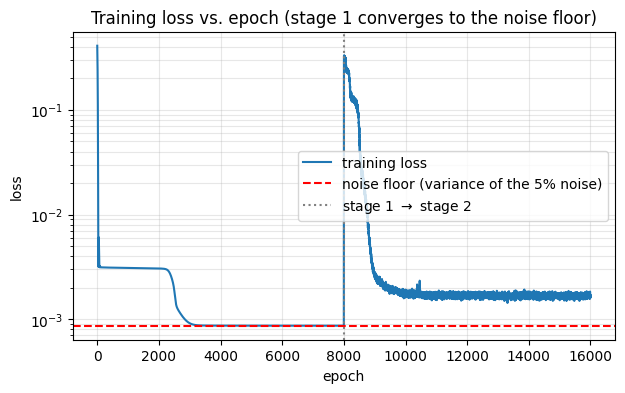
\includegraphics[width=\textwidth]{figures/PA__train_loss_epoch.png}
        \caption{Training loss vs.\ the noise floor.}
    \end{subfigure}
    %
    \begin{subfigure}[b]{0.48\textwidth}
        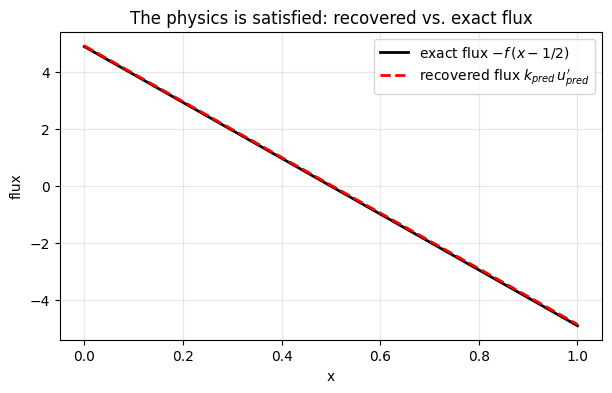
\includegraphics[width=\textwidth]{figures/PA_flux.png}
        \caption{Recovered vs.\ exact flux.}
    \end{subfigure}
    \caption{Problem A diagnostics: noise-floor convergence and flux consistency.}
    \label{fig:appnA_A}
\end{figure}

\section*{Problem B}
Figure~\ref{fig:appnA_B} localizes the $3.2\%$ error of the Deep Ritz
solution. Left: overlaying the phase interfaces (white contours) on the
pointwise error map shows that the error is organized in thin bands along
the material interfaces, as argued in Chapter~\ref{ch:problem_B}. Right: a
cross-section at $x_2 = 0.5$ makes the mechanism visible at the level of
the solution profile -- the reference pressure changes slope where the line
crosses an inclusion, and the smooth tanh ansatz follows the profile
closely while rounding off these kinks.
%
\begin{figure}[ht]
    \centering
    \begin{subfigure}[b]{0.48\textwidth}
        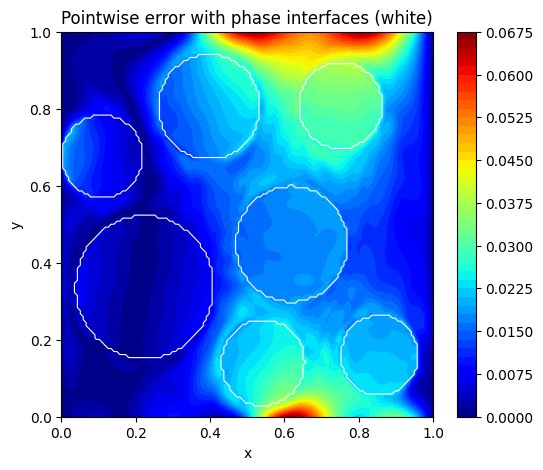
\includegraphics[width=\textwidth]{figures/PB_err_interfaces.png}
        \caption{Pointwise error with interfaces overlaid.}
    \end{subfigure}
    %
    \begin{subfigure}[b]{0.48\textwidth}
        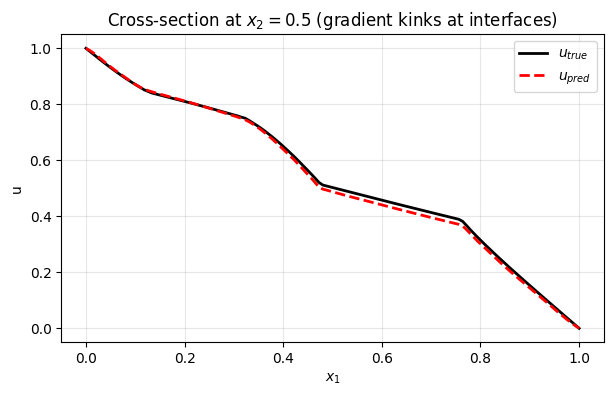
\includegraphics[width=\textwidth]{figures/PB_crossection.png}
        \caption{Cross-section at $x_2 = 0.5$.}
    \end{subfigure}
    \caption{Problem B diagnostics: the error is concentrated at the phase interfaces.}
    \label{fig:appnA_B}
\end{figure}

\section*{Problem C}
Figure~\ref{fig:appnA_C} characterizes the spread behind the mean test
error of the FNO. The histogram of the $200$ per-sample relative errors
shows a compact distribution around the mean rather than a few
catastrophic outliers, and the worst test sample (shown below the
histogram) remains qualitatively correct -- its error is elevated but of
the same character as the average case, concentrated near steep
conductivity gradients. Together these plots show that the reported mean
is representative of the operator's behaviour across the test
distribution.
%
\begin{figure}[ht]
    \centering
    \begin{subfigure}[b]{0.55\textwidth}
        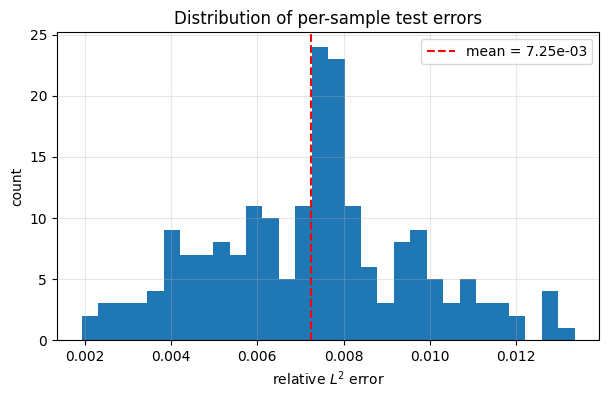
\includegraphics[width=\textwidth]{figures/PC_err_hist.png}
        \caption{Per-sample test error distribution.}
    \end{subfigure}
    \\[0.3cm]
    \begin{subfigure}[b]{0.98\textwidth}
        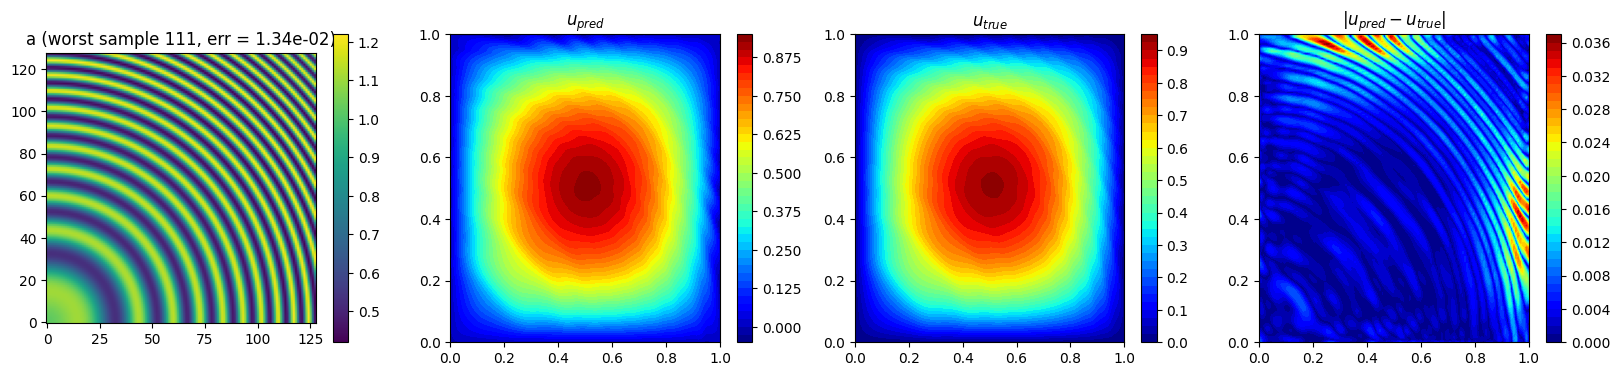
\includegraphics[width=\textwidth]{figures/PC_worst_sample.png}
        \caption{The worst test sample: input, prediction, reference, and pointwise error.}
    \end{subfigure}
    \caption{Problem C diagnostics: error distribution and worst-case behaviour.}
    \label{fig:appnA_C}
\end{figure}

\section*{Problem D}
Figure~\ref{fig:appnA_D} complements the space-time colour maps of
Chapter~\ref{ch:problem_D}. Left: solution profiles at $t = 0$, $0.25$,
$0.5$, and $1.0$ for the first test instance show that the PI-DeepONet
tracks the steepening and subsequent viscous decay of the front, with the
largest (still small) deviations at the steepest profile -- consistent
with the smooth basis expansion being least efficient there. Right: the
per-sample error histogram is right-skewed -- the bulk of the $200$ test
samples lies between $2\%$ and $5\%$ (the median is below the $4.1\%$
mean), while a small tail of harder samples reaches $10$--$14\%$ and a
single outlier about $25\%$. The tail samples are the initial conditions
that develop the steepest fronts, i.e.\ exactly the regime in which the
smooth DeepONet basis is weakest; this skew also means the mean error
reported in Chapter~\ref{ch:problem_D} is a conservative summary of the
typical case.
%
\begin{figure}[ht]
    \centering
    \begin{subfigure}[b]{0.48\textwidth}
        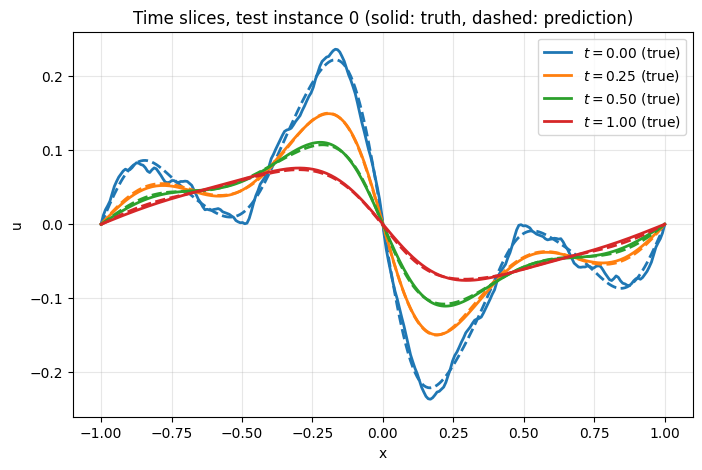
\includegraphics[width=\textwidth]{figures/PD_time_slices.png}
        \caption{Time slices: truth (solid) vs.\ prediction (dashed).}
    \end{subfigure}
    %
    \begin{subfigure}[b]{0.48\textwidth}
        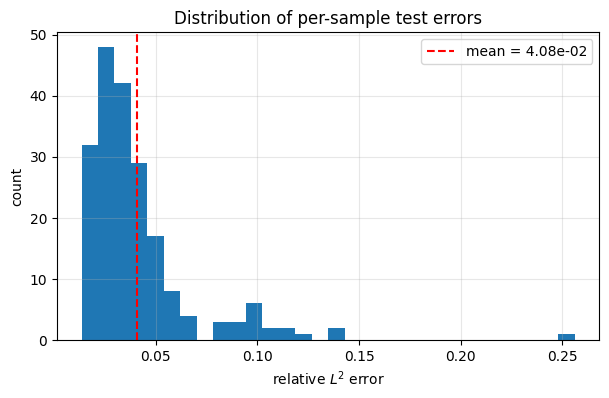
\includegraphics[width=\textwidth]{figures/PD_err_hist.png}
        \caption{Per-sample test error distribution.}
    \end{subfigure}
    \caption{Problem D diagnostics: front tracking and error distribution.}
    \label{fig:appnA_D}
\end{figure}
        % \input{chapters/appendix_B.tex}
    \end{appendices}
    
\end{document}
